\label{sec:learning}
\section{Learning Labels}

The creation of nutritional labels is often cast as a design problem rather than a computational problem~\cite{DBLP:journals/corr/abs-1803-09010,DBLP:journals/corr/abs-1805-03677}. Standard labels with broad applicability can amortize the cost of design, but the diversity of datasets, methods, and desirable properties for nutritional labels suggest a learning approach to help develop labels for a variety of situations. Since opaque automation is what motivated the need for labels in the first place, automating their creation may seem like a step backwards.  But there are several benefits:
\begin{itemize}
    \item Coverage: \emph{some} information provided in (nearly) \emph{all} cases is preferable to \emph{all} information provided in \emph{some} cases, as there are many models and datasets being deployed.
    \item Correctness: Hand-designed labels imply human metadata attachment, but curation of metadata is essentially an unsolved problem.  Computable labels reduce reliance on human curation efforts.
    \item Retroactivity: Some information can only be manually collected at the time of data collection (\eg demographics of authors in a speech corpus to control for nationality bias). This opportunity is lost for existing datasets.  However, inferring relevant properties based on the content of the data may be ``better than nothing.'' 
\end{itemize} 

We now consider two approaches to the problem of learning labels, one based on the visualization recommendation literature, and one based on bin-packing optimization.

\subsection{Learning as Visualization Recommendation}
Moritz et al. proposed Draco~\cite{2019-draco}, a formal model that represents visualizations as sets of logical facts, and represents design guidelines as a collection of hard and soft constraints over these facts, following an earlier proposal for the VizDeck system~\cite{DBLP:conf/sigmod/KeyHPA12}. Draco enumerates the visualizations that do not violate the hard constraints and finds the most preferred visualizations according to the weights of the soft constraints.  Formalized visualization descriptions are derived from the Vega-Lite grammar~\cite{DBLP:journals/tvcg/SatyanarayanMWH17} extended with rules to encode expressiveness criteria~\cite{DBLP:journals/tog/Mackinlay86}, preference rules validated in perception experiments, and general visualization design best practices. Hard constraints \emph{must} be satisfied (\eg shape encodings cannot express quantitative values), whereas soft constraints express a preference (\eg temporal values should use the x-axis by default). The weights associated with soft constraints can be learned from preference or utility data, when available (see example in Figure~\ref{fig:synthesis}).  

Draco implements the constraints using Answer Set Programming (ASP) semantics, and casts the problem of finding appropriate encodings as finding optimal answer sets~\cite{DBLP:phd/de/Gebser2011}. Draco has been extended to optimize for constraints over multiple visualizations~\cite{DBLP:journals/tvcg/QuH18}, and adapted for use in specialized domains.

\begin{figure}
    \centering
    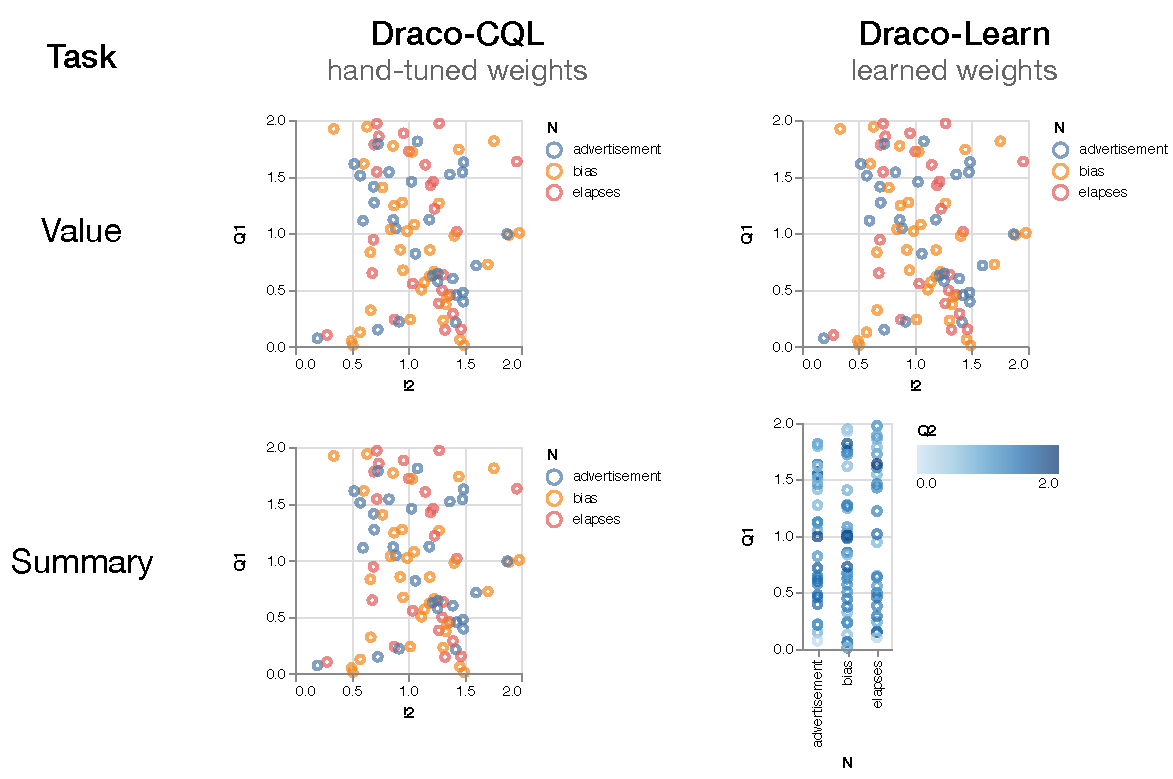
\includegraphics[width=0.65\columnwidth]{figs/synthesis}
    \vspace{-18pt}
    \caption{\label{fig:synthesis} Draco can be used to re-implement existing visualization systems like CQL by hand-tuning weights (left) or be used to learn weights automatically from preference data (right).  The visualizations selected can vary significantly, affording customization for specific applications.  A similar approach can be used when generating nutritional labels for data and models.}
    \vspace{-10pt}
\end{figure}

Using Draco (or similar formalizations), the specialized constraints governing the construction of nutritional labels can be developed in the general framework of ASP, while borrowing the foundational constraints capturing general visualization design principles. This approach can help reduce the cost of developing hundreds of application-specific labels by encoding common patterns, such as including descriptive statistics in all labels, or only showing fairness visualizations when bias is detected.

%Given a space of widgets such as those described in Section \ref{sec:rankingFacts}, the problem is to select...

\subsection{Learning as Optimization}
Sun et al. proposed MithraLabel~\cite{sun2019mithralabelJ}, focusing on generating task-specific labels for datasets to determine fitness for specific tasks. Considering the dataset as a collection of items over a set of attributes, each widget provides specific information (such as functional dependencies) about the whole dataset or some selected part of it. For example, if a data scientist is considering the use of a number-of-prior-arrests attribute to predict likelihood of recidivism, she should know that the number of prior arrests is highly correlated with the likelihood of re-offending, but it introduces bias as the number of prior arrests is higher for African Americans than for other races due to policing practices and segregation effects in poor neighborhoods. Widgets that might appear in the nutritional label for prior arrests include the  count of missing values, correlation with the predicted attribute or a protected attribute, and the distribution of values.